\section{Durchführung}
\label{sec:Durchführung}
\subsection{Messung unter  1 bar.}
\label{sec:p<1}
Der Aufbau der Apparatur entspricht der Abbildung \ref{abb:aufbau1}.
\begin{figure}
  \centering
  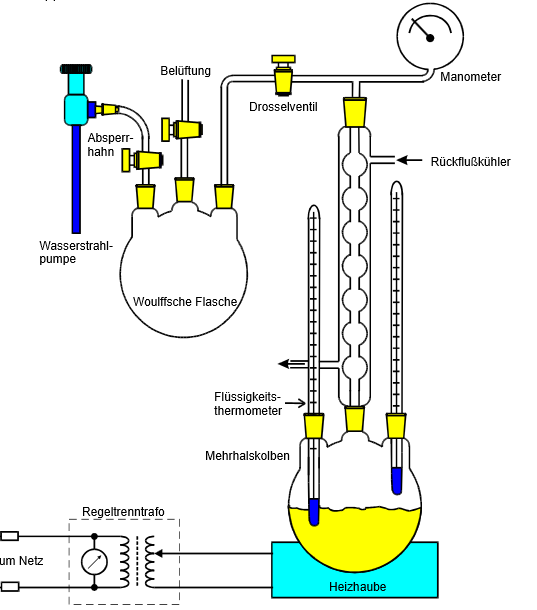
\includegraphics[width=0.7\textwidth]{aufbau1.PNG}
  \caption{Aufbau für die Messung bis 1 bar.}
  \label{abb:aufbau1}
\end{figure}\\
Zu Beginn wird die Apparatur evakuiert, dazu wird das
Belüftungsventil geschlossen und der Absperrhahn und das
Drosselventil geöffnet. Die Wasserstrahlpumpe wird angestellt
und solange angelassen bis sich ein konstanter Druk von ca. 40 mbar einstellt.
Drosselventil und Absperrhahn werden wieder verschlossen und die Heizhaube angeschaltet, um das Wasser im Mehrhalskolben zu erhitzen.
Die Wasserkühlung wird angestellt, um den entstehenden Wasserdampf zu kondensieren.
Es werden die Wertepaare der Temperatur und des Druckes im Gasraum aufgenommen,
bis sich im Inneren ein Druck von ca. 1 bar eingestellt hat.
\newpage
\subsection{Messung über 1 bar.}
\begin{figure}
  \centering
  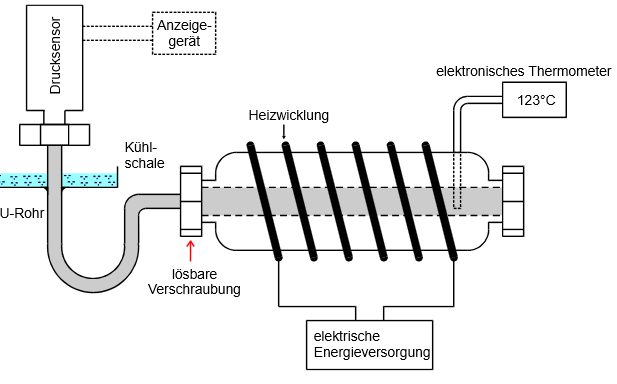
\includegraphics[width=0.7\textwidth]{aufbau2.PNG}
  \caption{Aufbau für die Messung zwischen 1 und 15 bar.}
  \label{abb:aufbau2}
\end{figure}
In Abbildung \ref{abb:aufbau2} ist der Aufbau für die Messung dargestellt. Im Inneren der Apparatur befindet sich bereits Wasser.
Die Kühlschale wird mit Wasser aufgefüllt und das Heizelement eingeschaltet.
Temperatur und entsprechender Druck werden notiert bis ein Druck von ungefähr 15 bar erreicht wird.
